
%(BEGIN_QUESTION)
% Copyright 2014, Tony R. Kuphaldt, released under the Creative Commons Attribution License (v 1.0)
% This means you may do almost anything with this work of mine, so long as you give me proper credit

Examine this schematic of a liquid level control system for an open vessel:

$$\includegraphics[width=15.5cm]{i04717x01.eps}$$

Determine the effect on the control system's regulation of liquid level inside the vessel if the incoming liquid flow rate suddenly decreases.  Assume all loop components are properly configured, that the controller is well-tuned, and that a significant amount of time has passed since the feed flow rate decreased.  Compare these conditions with what they were before the process change:

\begin{itemize}
\item{} Liquid level will: {\it increase} from what it was before, {\it decrease} from what it was before, or {\it remain the same} as before
\vskip 10pt
\item{} Control valve will: {\it open up} further, {\it close down} more, or {\it remain in the same position} 
\end{itemize}

\underbar{file i04717}
%(END_QUESTION)





%(BEGIN_ANSWER)

\begin{itemize}
\item{} Liquid level will: {\bf remain the same as before}
\vskip 10pt
\item{} Control valve will: {\bf close down more}
\end{itemize}

%(END_ANSWER)





%(BEGIN_NOTES)

{\bf This question is intended for exams only and not worksheets!}.

%(END_NOTES)

